\begin{figure*}[h!]
	\vspace{-.1in}
	\begin{center}
		\begin{tabular}{ c  c  c  c  c  }
			%\hline
			%\large{\textsf{17:12 GST}}  &   \large{\textsf{20:08 GST}}   &\large{\textsf{23:12 GST}} &\large{\textsf{02:08 GST}}  &\large{\textsf{05:18 GST}}    \\
			\large{\textsf{17 GST / 0 Hrs}}  &   \large{\textsf{20 GST / 3 Hrs}}   &\large{\textsf{23 GST / 6 Hrs}} &\large{\textsf{2 GST / 9 Hrs}}  &\large{\textsf{6 GST / 13 Hrs}}    \\
			%\small{\textsf{0 Hrs}}  &   \small{\textsf{3 Hrs}}   &\small{\textsf{6 Hrs}} &\small{\textsf{9 Hrs}}  &\small{\textsf{12 Hrs}}    \\
			{{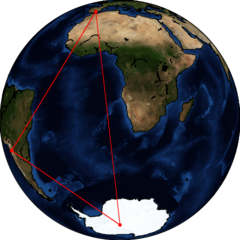
\includegraphics[width=.17\linewidth]{figures/uvcoverage/frames4/spin004.png}} }  & {{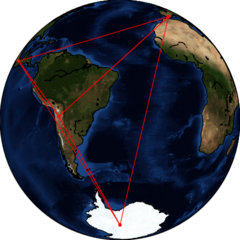
\includegraphics[width=.17\linewidth]{figures/uvcoverage/frames4/spin040.png}} } &
			{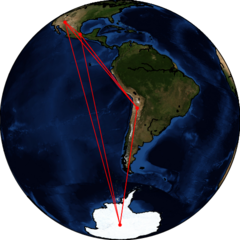
\includegraphics[width=.17\linewidth]{figures/uvcoverage/frames4/spin074.png}} %76
			&
			{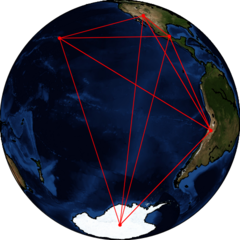
\includegraphics[width=.17\linewidth]{figures/uvcoverage/frames4/spin111.png}} &
			{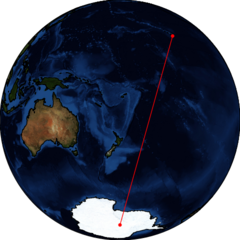
\includegraphics[width=.17\linewidth]{figures/uvcoverage/frames4/spin159.png}} %147.png}} 
			
			\\
			\Large{$\Downarrow$}  &   \Large{$\Downarrow$}  & \Large{$\Downarrow$} & \Large{$\Downarrow$}& \Large{$\Downarrow$}     \\
			& \vspace{-.1in}
			\\
			{{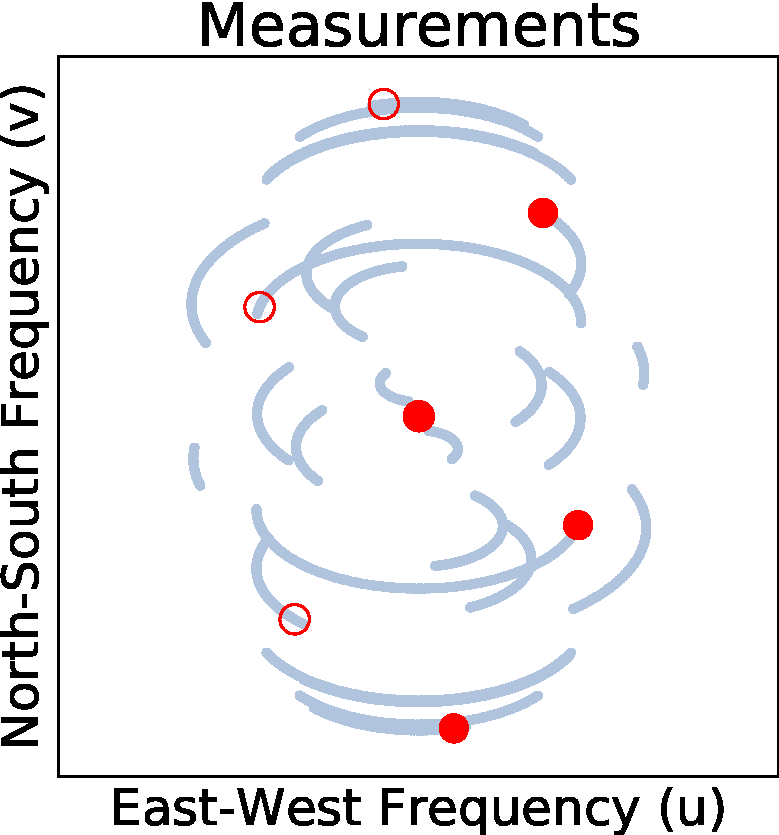
\includegraphics[width=.17\linewidth]{figures/uvcoverage/frames4/uv_singleptbig_merge_4.pdf}} } &
			{{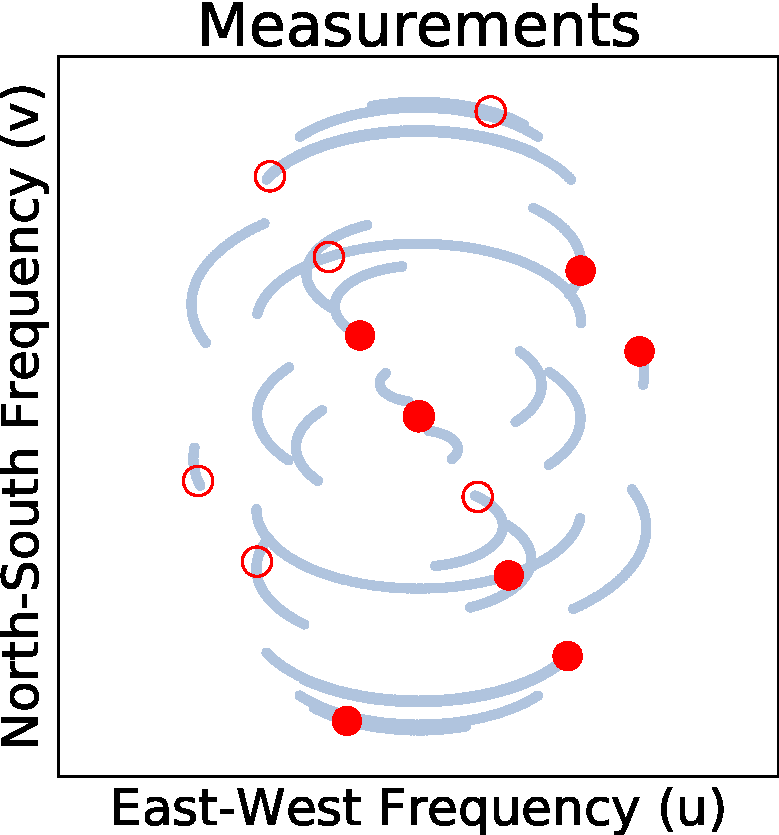
\includegraphics[width=.17\linewidth]{figures/uvcoverage/frames4/uv_singleptbig_merge_40.pdf}} } &
			{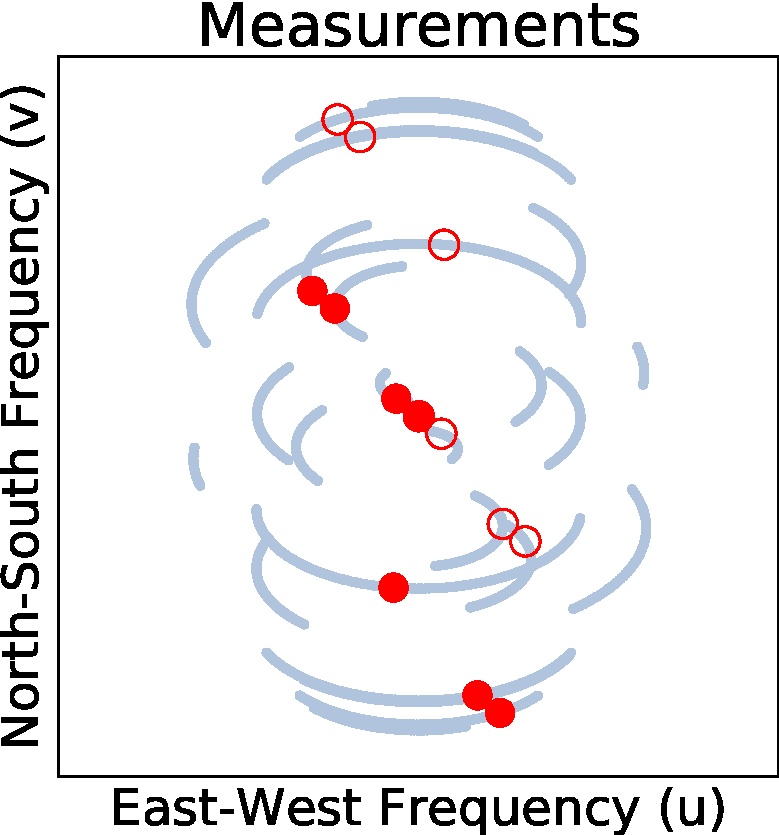
\includegraphics[width=.17\linewidth]{figures/uvcoverage/frames4/uv_singleptbig_merge_74.pdf}} %76 
			&
			{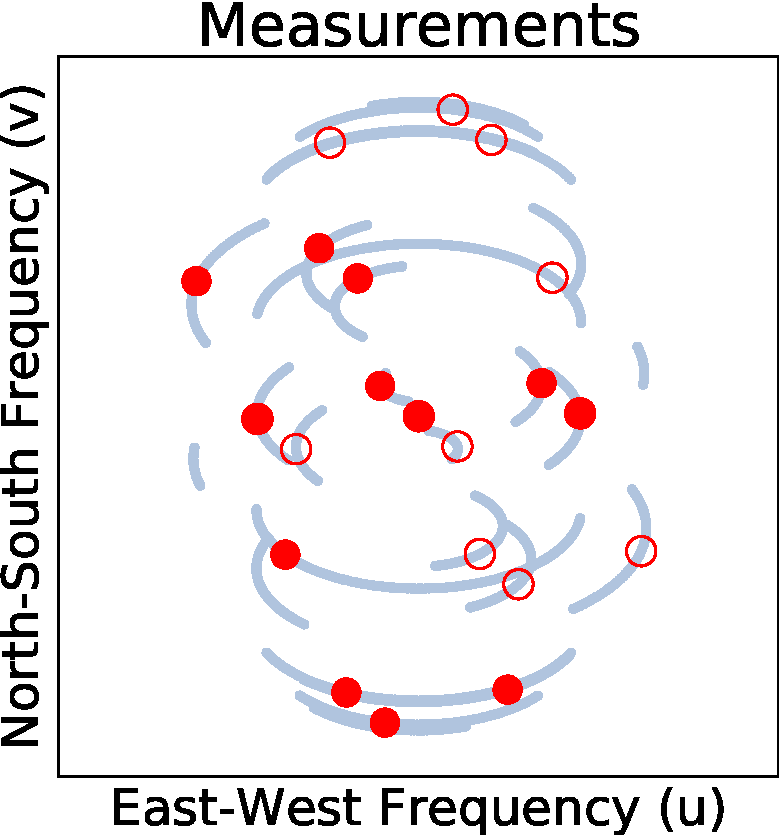
\includegraphics[width=.17\linewidth]{figures/uvcoverage/frames4/uv_singleptbig_merge_111.pdf}} &
			{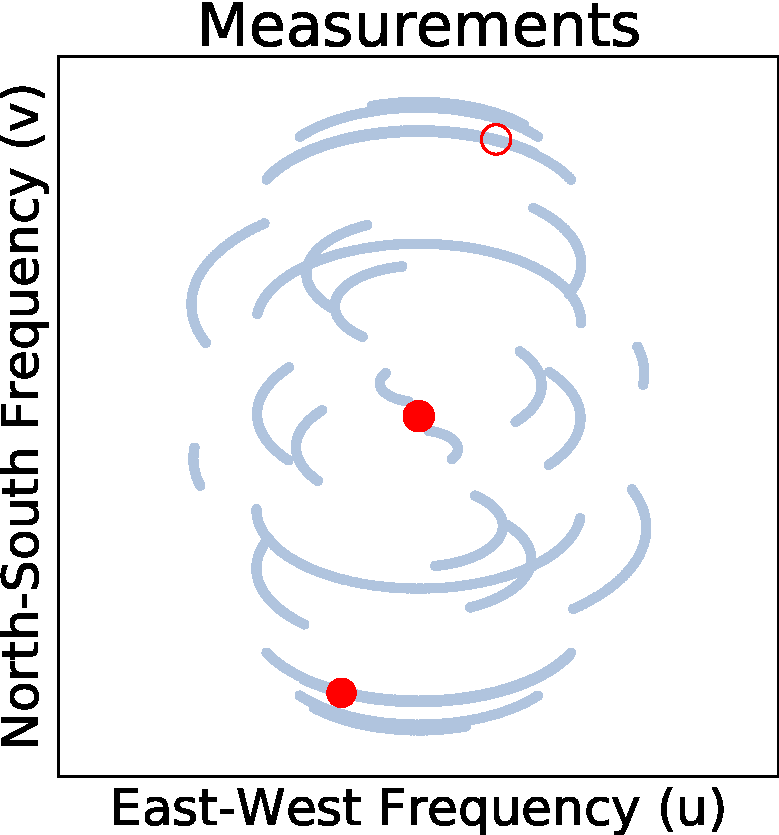
\includegraphics[width=.17\linewidth]{figures/uvcoverage/frames4/uv_singleptbig_merge_159.pdf}} %147.png}} 
			\\
		\end{tabular}
		\caption{{\bf Earth Rotation Synthesis:} For every two telescopes in the interferometric array, we obtain a single measurement (visibility) related to the underlying source image's 2D spatial frequency. This frequency is related to the baseline between the telescopes in the direction perpendicular to the observing source. 
			%This would be a prohibitively small number of measurements to make an image from. 
			It is prohibitively difficult to reconstruct a faithful image from just these small number of measurements. 
			However, as the Earth rotates, the projected baselines change, and we observe new measurements related to different regions of the 2D frequency plane. 
			As time progresses (specified by the Greenwich Sidereal Time (GST)), the projected baselines change and the red dots on the frequency coverage plot (bottom row), which indicate the current measurements, change position. 
			Assuming the source is static, this amounts to carving out elliptical paths in the frequency plane that are all related to the same image. The set of all frequencies sampled over an observation is shown by the transparent blue lines. However, when a source evolves over the course of a night's observation, each instantaneous set of measurements (shown in red on each frequency plot) is only related to a single image.
			As light emitted from the source is real-valued we obtain two measurements on opposite sides of the frequency plane -- each independent set of measurements displayed as either the open or closed red circles. The Earth diagrams are shown from the point of view of an observer at Sgr A*. Note that although the telescope array is not changing, the number of visibilities at a given time changes depending on how many sites can still see Sgr A*. 
			%In this work we present a way to join these measurements in order to reconstruct a video of the emission, rather than a single image. 
		} 
		\label{fig:earthrotationsythesis}
	\end{center}
	\vspace{-.1in}
\end{figure*}


\vspace{-.1in}
\section{Introduction}

Imaging distant astronomical sources with high resolving power at radio wavelengths would require single-dish telescopes with prohibitively large diameters due to the inverse relationship between angular resolution and telescope diameter. Very long baseline interferometry (VLBI) is a technique that alleviates the need for building an impossibly large single-dish telescope by simultaneously observing a common source from an array of telescopes distributed around the Earth. This technique makes it possible to emulate samples from a single-dish telescope with a diameter equal to the maximum distance between telescopes in the array, at the expense of having to handle missing data~\cite{TMS}. Thus far, VLBI has been primarily used to image sources that are static on the time scale of a day's observation. In this work, we extend the technique's applicability to imaging time-varying sources by reconstructing a video of the source. % rather than a single image. 

VLBI measurements place a sparse set of constraints on
the %emission 
spatial frequencies of the underlying source image. In particular, each pair of telescopes provides information about a single 2D spatial frequency. This frequency is related to the baseline vector connecting the two telescope sites, projected orthogonal to the direction of the target source~\cite{TMS}. Thus, at a single time, for an array with $\ntele$ telescopes, at most ${\ntele (\ntele - 1)}/{2}$ spatial frequencies are measured. 
For example, an array of 6 telescopes would yield only 15 measurements. 
%This would result in only 15 measurements for an array of 6 telescopes. % measurements. 
% corresponding to each pair of telescopes. 
%For a small telescope array this is an incredibly small number of spatial frequencies to reconstruct an image from. 
However, as the Earth rotates, 
the baseline vector connecting each pair of telescopes changes. This allows the array to sample additional spatial frequencies along elliptical paths in the frequency domain~\cite{TMS}. Refer to Figure~\ref{fig:earthrotationsythesis}. Combining the different measurements taken as the Earth rotates is referred to as {\it Earth Rotation Synthesis}.
Earth rotation synthesis 
is essential for building up enough measurements to constrain image reconstruction.

The task of reconstructing an image from these sparse constraints is highly ill-posed and relies heavily on assumptions made about the underlying image~\cite{hogbom1974aperture, taylor1999synthesis, rusenimaging}. 
%image priors and assumptions about the observational process. 
%Reconstructing an image using VLBI measurements is an ill-posed problem, and as such each there are an infinite number of possible images that explain the data. 
%The challenge is to find an explanation that respects our prior assumptions about what images look like, while still satisfying the observed data.
%For a small telescope array there are too few measurements to reconstruct an image from a single time. 
%Earth rotation synthesis is essential for building up enough measurements to constrain image reconstruction.
If a source is static, the VLBI measurements -- taken over time as the Earth rotates -- all correspond to the same underlying image. 
Under a static source assumption, 
%The task of reconstructing an image from these sparse constraints is highly ill-posed and relies heavily on priors to guide optimization. 
recently developed VLBI image reconstruction techniques have been demonstrated on small telescope arrays~\cite{bouman2016computational, andrew, kazu, Fish_2016_Imaging, akiyama2017superresolution}.
%recently developed VLBI image reconstruction techniques perform reasonably well, even with a small telescope array. 
%been reasonably successful in imaging static astronomical sources with a small telescope array. 
%using Earth-rotation synthesis. 
However, for an evolving source, measurements are no longer sampled from the same image, and these reconstruction algorithms quickly break down. 



%In a static source, the measurements taken over time as the Earth rotates all correspond to the same underlying image. 
%However, for an evolving source, these measurements through time do not correspond to the same image, and thus are sampled from different emission images. 


%For a static source, the VLBI measurements -- taken over time as the Earth rotates -- all correspond to the same underlying image. 
%However, for an evolving source, these measurements are sampled from different emission images. 
%In a static source, the measurements -- taken over time as the Earth rotates -- all correspond to the same underlying image.  
Although most %Nearly all 
astronomical sources are static over the time scale of a night's observation, 
%This static source assumption is reasonable for nearly all astrophysical sources. 
%However, 
some notable
%notable
sources have detectable structural changes on much shorter timescales. 
For instance,  the Galactic Center supermassive black hole, Sagittarius A* (SgrA*), has an estimated mass of only four-million solar masses~\cite{Ghez_2008}. %, resulting in a gravitational timescale, $GM/c^3$, of just 20 seconds.
%For instance,  the Galactic Center supermassive black hole, Sagittarius A* (SgrA*), evolves on the timescale of minutes. 
%Because SgrA* has an estimated mass of only four-million solar masses, its gravitational timescale $GM/c^3$ is just 20 seconds. 
This implies that SgrA* is quickly evolving, with an innermost stable circular orbit of just 4 to 30 minutes, depending on the spin of the black hole~\cite{orbitalperiod}. 
%\katie{mention magnetorotational-instability-driven turbulence?}
Previous observations have shown that SgrA* varies dramatically over a night's observation on the scale of its predicted event horizon, in both total-intensity and polarization~\cite{Fish_2011, Johnson_2015}. 
%This time-variation has been observed on both total-intensity and polarization observations made of SgrA* to date.  
%Dynamic sources such as SgrA* (a prime target for the Event Horizon Telescope) do not agree with this assumption. Simulations and polarization have shown that SgrA* changes dramatically over the time period of just a few hours. 

SgrA* is a prime target for the Event Horizon Telescope (EHT) -- an international project whose goal is to take the first image of the immediate environment around a black hole~\cite{Doeleman_2009}.
Realizing this goal would not only substantiate the existence of a black holes' event horizon, but also aid in studying general relativity in the strong field regime~\cite{Doeleman_2008, Johannsen_2010}.
Unfortunately, the amount of variation predicted for SgrA* suggests that conventional VLBI imaging techniques will be inappropriate for observations taken by the EHT~\cite{rusenimaging,orbitalperiod}. 
%Having the level of variation seen in SgrA* over a single observation is challenging from 
%This can be challenging from 
%an imaging perspective. 
%As the measurements are taken from different underlying emission images, imaging algorithms can no longer be collapsed to solving for a single image that explains all of the collected data. 
%Most interferometric imaging algorithms assume the source being observed is static. 
%However, in the case of dynamic sources, such as SgrA*, the assumptions of a static source no longer hold. 
Thus, in this work we present a new imaging algorithm for time-varying sources that models the VLBI observations as being from a Gaussian Markov Model. % that we believe will help in imaging SgrA*. 
Our dynamic imaging algorithm allows for an evolving emission region by simultaneously reconstructing both images and motion trajectories - essentially reconstructing a video rather than a static image.

In Section~\ref{sec:meas} we review the basics of interferometric imaging and the data traditionally used to constrain image reconstruction. In Section~\ref{sec:setup} we summarize standard approaches to VLBI imaging and define a generalized expression for data consistency. In Section~\ref{sec:static} we explain how static imaging can be performed under a multivariate Gaussian prior. Highlighting the approach's benefits first in the case of a static source becomes helpful when discussing our proposed solution to the more complex dynamic imaging problem, StarWarps, in Section~\ref{sec:dynamic_model}, and when deriving our proposed EM inference algorithm in Section~\ref{sec:dynamic_inference}. Results can be seen in Section~\ref{sec:results}, followed by concluding remarks in Section~\ref{sec:conclusion}.


%For example, using simulated observations of a \hot spot" orbiting Sgr A (Broderick & Loeb 2005, 2006), Doeleman et al. (2009b) and Fish et al. (2009) demonstrated that robust VLBI observables such as closure phase and fractional polarization can sensitively detect periodicities associated with these hot spots.
